\section{Weight Initialization}

  The way that we initialize our weights can have a huge impact on our training performance. Imagine that you are creating the first neural network and you want to decide how to initialize it. You may consider many different cases. 

  \begin{example}[Constant Initialization]
    You may first think of initializing everything to $0$ or $1$, which is the simplest. Let's run this, but we can already see by epoch 15 that we have some problems. 
    \begin{center}
      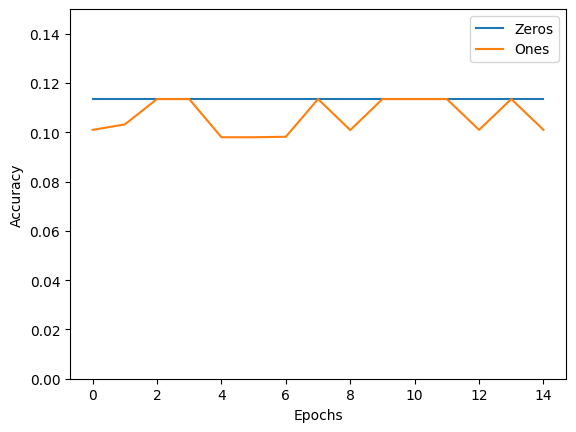
\includegraphics[scale=0.5]{img/first_initialize.png}
    \end{center}
    Clearly, this is not good, and theoretically this makes sense since it means all our activations are going to be the same, and thus all our gradients will be the same, meaning that are updates will be the same for every weight, which is not good mixing. We can see this below: 
  \end{example}

  \begin{example}[Random Initialization with High Variance]
    Okay, this didn't work, so perhaps you think it would be a good idea have more randomness to the initialization so that all the weights aren't exactly one number. You could think of initializing everything with three distinct schemes: 
    \begin{enumerate}[itemsep=0mm] 
      \item Randomly initialize everything to be $-1$ or $1$ with equal probability. 
      \item Randomly initialize everything to be a Gaussian random variable with standard deviation $1$. 
      \item Randomly initialize everything to be a uniform random variable between $-1$ and $1$. 
    \end{enumerate}
    Running the experiments give the following. 
    \begin{center} 
      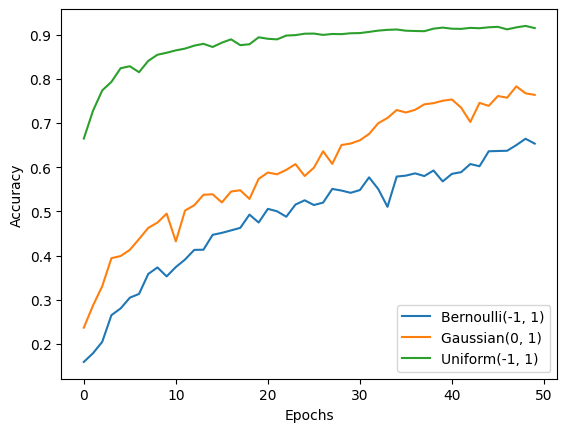
\includegraphics[scale=0.5]{img/second_initialization.png}
    \end{center}
    However, this is also not good since it means that the activations will be very large, and thus the gradients will be very large, and so the updates will be very large. This is not good since it means that the weights will be jumping around a lot, and we won't be able to converge. Furthermore, depending on what activations we choose, e.g. tanh or sigmoid, very large activations may saturate the gradients and kill the learning. 
  \end{example}

  \begin{example}[Random Initialization with Low Variance]
    This improves the next problem but now you want to fix the situation of the gradients being too big. Therefore, you should initialize the parameters to be smaller values, but not so small that they are zeros and we have the same problem as before. We use improved schemes: 
    \begin{enumerate}[itemsep=0mm] 
      \item Randomly initialize everything to be $-0.1$ or $0.1$ with equal probability. 
      \item Randomly initialize everything to be a Gaussian random variable with standard deviation $0.1$. 
      \item Randomly initialize everything to be a uniform random variable between $-0.1$ and $0.1$.
    \end{enumerate}
    \begin{center}
      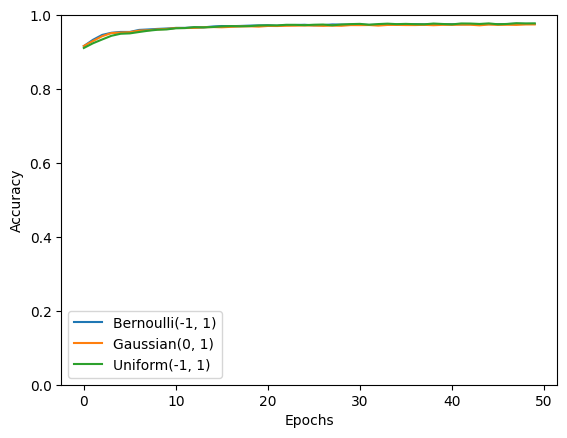
\includegraphics[scale=0.5]{img/third_initialize.png}
    \end{center}
  \end{example}

  Through out experiments, we have learned that a good rule of thumb for initializing weights is to make them small and uniformly random without being too small. While it is harder to get better than this for MNIST, a slightly better approach is Xavier initialization, which builds upon our same ideas. 

  \begin{definition}[Xavier Initialization]
    The \textbf{Xavier initialization} simply initializes each weight as a uniform distribution, with its range dependent on the size of the input. 
    \begin{equation}
      w_{ij}^{[l]} \sim U \bigg( -\frac{1}{\sqrt{N^{[l-1]}}}, \frac{1}{\sqrt{N^{[l-1]}}} \bigg)
    \end{equation}
    where $N^{[l-1]}$ is the number of neurons in the previous layer. This is a good rule of thumb for the weights, but the biases can be initialized to $0$ (though they are also initialized uniformly by default).
  \end{definition}

  \begin{code}[Experimenting with Weight Initializations] 
    The code used for generating the figures can be found \href{code/initialization.ipynb}{here}. 
  \end{code}

